%%%%%%%%%%%%%%%%%%%%%%%%%%%%%%%%%%%%%%%%%%%%%%%%%%%%%%%%%%%%%%%
%
% Welcome to writeLaTeX --- just edit your LaTeX on the left,
% and we'll compile it for you on the right. If you give
% someone the link to this page, they can edit at the same
% time. See the help menu above for more info. Enjoy!
%
%%%%%%%%%%%%%%%%%%%%%%%%%%%%%%%%%%%%%%%%%%%%%%%%%%%%%%%%%%%%%%%

% --------------------------------------------------------------
% This is all preamble stuff that you don't have to worry about.
% Head down to where it says "Start here"
% --------------------------------------------------------------
 
\documentclass[12pt]{article}
 
\usepackage[margin=1in]{geometry}
\usepackage{amsmath,amsthm,amssymb}
\usepackage{siunitx}

\usepackage{listings}
\usepackage{xcolor}
\usepackage{circuitikz}
\usetikzlibrary{bending}
\usetikzlibrary{patterns,decorations.pathmorphing,positioning}
\usepackage{enumitem}

\usepackage{tikz}
\usetikzlibrary{shapes,arrows,positioning,calc}
\tikzset{
block/.style = {draw, fill=white, rectangle, minimum height=3em, minimum width=3em},
tmp/.style  = {coordinate}, 
sum/.style= {draw, fill=white, circle},
input/.style = {coordinate},
output/.style= {coordinate},
pinstyle/.style = {pin edge={to-,thin,black}
}
}

\usepackage{float,graphicx}

%New colors defined below
\definecolor{codegreen}{rgb}{0,0.6,0}
\definecolor{codegray}{rgb}{0.5,0.5,0.5}
\definecolor{codepurple}{rgb}{0.58,0,0.82}
\definecolor{backcolour}{rgb}{0.95,0.95,0.92}

%Code listing style named "mystyle"
\lstdefinestyle{mystyle}{
  backgroundcolor=\color{backcolour}, commentstyle=\color{codegreen},
  keywordstyle=\color{magenta},
  numberstyle=\tiny\color{codegray},
  stringstyle=\color{codepurple},
  basicstyle=\ttfamily\footnotesize,
  breakatwhitespace=false,         
  breaklines=true,                 
  captionpos=b,                    
  keepspaces=true,                 
  numbers=left,                    
  numbersep=5pt,                  
  showspaces=false,                
  showstringspaces=false,
  showtabs=false,                  
  tabsize=2
}

%"mystyle" code listing set
\lstset{style=mystyle}

 
\newcommand{\N}{\mathbb{N}}
\newcommand{\Z}{\mathbb{Z}}
 
\newenvironment{theorem}[2][Theorem]{\begin{trivlist}
\item[\hskip \labelsep {\bfseries #1}\hskip \labelsep {\bfseries #2.}]}{\end{trivlist}}
\newenvironment{lemma}[2][Lemma]{\begin{trivlist}
\item[\hskip \labelsep {\bfseries #1}\hskip \labelsep {\bfseries #2.}]}{\end{trivlist}}
\newenvironment{exercise}[2][Exercise]{\begin{trivlist}
\item[\hskip \labelsep {\bfseries #1}\hskip \labelsep {\bfseries #2.}]}{\end{trivlist}}
\newenvironment{problem}[2][Problem]{\begin{trivlist}
\item[\hskip \labelsep {\bfseries #1}\hskip \labelsep {\bfseries #2.}]}{\end{trivlist}}
\newenvironment{question}[2][Question]{\begin{trivlist}
\item[\hskip \labelsep {\bfseries #1}\hskip \labelsep {\bfseries #2.}]}{\end{trivlist}}
\newenvironment{corollary}[2][Corollary]{\begin{trivlist}
\item[\hskip \labelsep {\bfseries #1}\hskip \labelsep {\bfseries #2.}]}{\end{trivlist}}

\newenvironment{solution}{\begin{proof}[Solution]}{\end{proof}}
 
\begin{document}
 
% --------------------------------------------------------------
%                         Start here
% --------------------------------------------------------------
 
\title{Homework 6}%replace X with the appropriate number
\author{Mengxiang Jiang\\ %replace with your name
EEEN 5338 Digital and DSP Based Control} %if necessary, replace with your course title
 
\maketitle
 
\begin{problem}{1} %You can use theorem, exercise, problem, or question here.  Modify x.yz to be whatever number you are proving
    A lead compensator is designed for a unity-feedback system whose plant transfer function is:
    $$ G_p(s) = \frac{100K}{s(s+36)(s+1000)}$$
    The design specifications are:\\
    Percent overshoot = 20\%\\
    Peak time = 0.1 seconds\\
    $K$ = 1440\\
    The lead compensator is:
    $$ G_c(s) = 2.38\left(\frac{s+25.3}{s+60.2}\right)$$
    If the system is to be computer controlled:\\
    \begin{enumerate}
        \item Find the digital controller, $G_c(z)$, assume: $T = 0.001$ seconds. 
        \begin{align*}
            \text{substitute } s = \frac{2(z-1)}{0.001(z+1)} \text{ into } G_c(s):\\
            G_c(z) = 2.38\left(\frac{2(z-1)+0.0253(z+1)}{0.001(z+1)}\right)\left(\frac{0.001(z+1)}{2(z-1)+0.0602(z+1)}\right)\\
            G_c(z) = 2.38\left(\frac{2.0253z - 1.9747}{2.0602z - 1.9398}\right) = 2.38\left(\frac{2.0253}{2.0602}\right)\left(\frac{z - 0.9750}{z-0.9416}\right)=2.3397\left(\frac{z - 0.9750}{z-0.9416}\right)
        \end{align*}
        \pagebreak
        \item Find the $z$-transform of the plant and the zero-order hold with $T=0.001$ seconds.
        \begin{figure}[H]
            \centering
            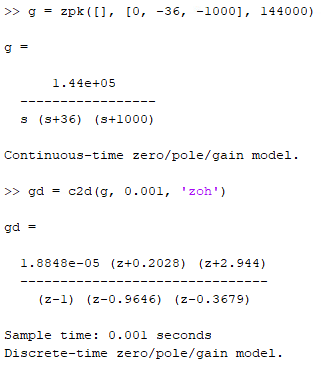
\includegraphics{2}
        \end{figure}
        Expanding the expression leads to:
        $$G_p(z) = \frac{\num{1.8848e-5}z^2+\num{5.9310e-5}z + \num{1.1253e-5}}{z^3-2.3325z^2+1.6874z-0.3549}$$
        \pagebreak
        \item Revise the MATLAB code (as per our class discussion in the examples from Lecture Notes 6) to solve and plot the step response for this system. Make sure to submit the code, the results, and the plot.
        \begin{figure}[H]
            \centering
            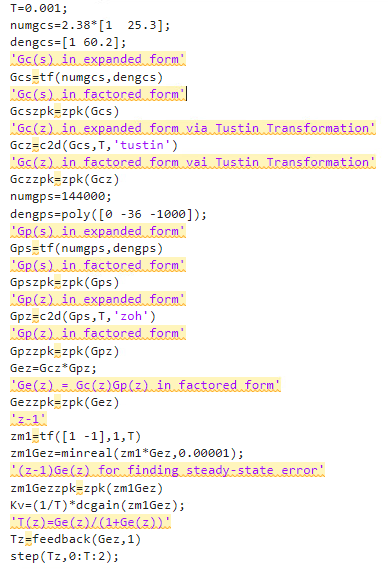
\includegraphics{3code}
            \caption{MATLAB code}
        \end{figure}
        \pagebreak
    \begin{lstlisting}[caption=MATLAB results]     
ans =

'Gc(s) in expanded form'


Gcs =

2.38 s + 60.21
--------------
 s + 60.2

Continuous-time transfer function.


ans =

'Gc(s) in factored form'


Gcszpk =

2.38 (s+25.3)
-------------
(s+60.2)

Continuous-time zero/pole/gain model.


ans =

'Gc(z) in expanded form via Tustin Transformation'


Gcz =

2.34 z - 2.281
--------------
z - 0.9416

Sample time: 0.001 seconds
Discrete-time transfer function.


ans =

'Gc(z) in factored form vai Tustin Transformation'


Gczzpk =

2.3397 (z-0.975)
----------------
 (z-0.9416)

Sample time: 0.001 seconds
Discrete-time zero/pole/gain model.


ans =

'Gp(s) in expanded form'


Gps =

       144000
------------------------
s^3 + 1036 s^2 + 36000 s

Continuous-time transfer function.


ans =

'Gp(s) in factored form'


Gpszpk =

  1.44e+05
-----------------
s (s+1000) (s+36)

Continuous-time zero/pole/gain model.


ans =

'Gp(z) in expanded form'


Gpz =

1.885e-05 z^2 + 5.931e-05 z + 1.125e-05
---------------------------------------
z^3 - 2.333 z^2 + 1.687 z - 0.3549

Sample time: 0.001 seconds
Discrete-time transfer function.


ans =

'Gp(z) in factored form'


Gpzzpk =

1.8848e-05 (z+2.944) (z+0.2028)
-------------------------------
(z-1) (z-0.9646) (z-0.3679)

Sample time: 0.001 seconds
Discrete-time zero/pole/gain model.


ans =

'Ge(z) = Gc(z)Gp(z) in factored form'


Gezzpk =

4.4097e-05 (z+2.944) (z-0.975) (z+0.2028)
-----------------------------------------
(z-1) (z-0.9646) (z-0.9416) (z-0.3679)

Sample time: 0.001 seconds
Discrete-time zero/pole/gain model.


ans =

'z-1'


zm1 =

z - 1

Sample time: 0.001 seconds
Discrete-time transfer function.


ans =

'(z-1)Ge(z) for finding steady-state error'


zm1Gezzpk =

4.4097e-05 (z+2.944) (z-0.975) (z+0.2028)
-----------------------------------------
  (z-0.9646) (z-0.9416) (z-0.3679)

Sample time: 0.001 seconds
Discrete-time zero/pole/gain model.


ans =

'T(z)=Ge(z)/(1+Ge(z))'


Tz =

4.41e-05 z^3 + 9.577e-05 z^2 - 0.000109 z - 2.566e-05
-----------------------------------------------------
 z^4 - 3.274 z^3 + 3.884 z^2 - 1.944 z + 0.3341

Sample time: 0.001 seconds
Discrete-time transfer function.
\end{lstlisting}
        \begin{figure}[H]
            \centering
            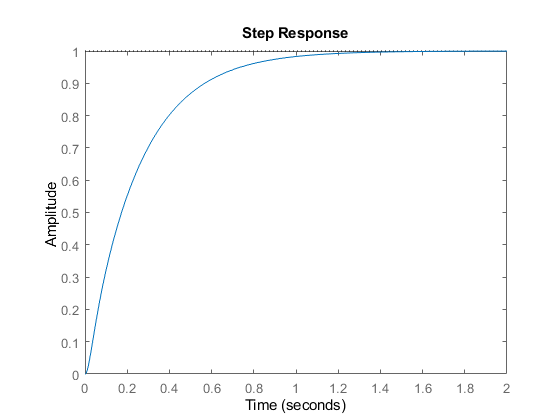
\includegraphics{3step}
            \caption{MATLAB plot}
        \end{figure}
    \end{enumerate}
\end{problem}

% --------------------------------------------------------------
%     You don't have to mess with anything below this line.
% --------------------------------------------------------------
 
\end{document}